% Preambuła
\documentclass[a4paper,11pt]{article}
\usepackage[polish]{babel}
\usepackage[OT4]{fontenc}
\usepackage[utf8]{inputenc}
\usepackage{geometry}
\usepackage{fancyhdr}
\usepackage{minted}
\usepackage{graphicx}

\geometry{lmargin=2cm}
\pagestyle{fancy}
\lhead{ZBD - zadanie 1}
\rhead{Piotr Zalas}

% Część główna
\begin{document}

{\bf Program 1} \\

Pomiar przeprowadziłem na swoim domowym komputerze. Wykorzystałem następujące nośniki pamięci:
\begin{enumerate}
	\item{Dysk wbudowany w komputer - Hitachi Travelstar 5K750 - EXT4}
	\item{Dysk zewnętrzny - Samsung S2 Portable - FAT}
	\item{Pamięć typu flash - Kingston DataTraveler 2.0 - FAT}
\end{enumerate}
Do przeprowadzenia pomiaru wykorzystałem poniższy program. Ilość operacji dyskowych wyznaczałem
eksperymentalnie w taki sposób, by czas pomiaru był obrobinę niższego rzędu niż wiek wszechświata.
W przypadku zapisów dane nie były generowane losowo gdyż funkcja rand() ma skłonność do zawieszania
się na dłuższą chwilę (nawet kilka sekund) co psuło wyniki pomiarów. Zamiast tego na dysk zrzucałem
dopiero co odczytany blok.

\inputminted[
frame=lines,
framesep=2mm,
baselinestretch=1.2,
fontsize=\footnotesize,
linenos
]{cpp}{iotest.cpp}

Wyniki wraz z przyjętymi parametrami obrazują poniższe tabele. Założyłem, że na każde 100 odczytanych
bloków przypada 1 zapisany blok. Operacja do wykonania w danej chwili jest wybierana losowo. \\

Odczyt z buforowaniem systemu plików:\\
\begin{tabular}{|l|l|l|l|l|l|} \hline
	Nośnik & Odczyty & Zapisy & Po ile bloków & Czas testu ($\mu s$) & Średni czas operacji ($\mu s$)\\
	\hline \hline
	Hitachi & 1000000 & 10000 & 1 & 2067758 & 2.047\\ \hline
	Samsung & 1000000 & 10000 & 1 & 1640246 & 1.624\\ \hline
	Kingston & 1000000 & 10000 & 1 & 1650492 & 1.634\\ \hline
	\hline
	Hitachi & 1000000 & 10000 & 10 & 1507583 & 1.492\\ \hline
	Samsung & 1000000 & 10000 & 10 & 1428341 & 1.414\\ \hline
	Kingston & 1000000 & 10000 & 10 & 1535337 & 1.520\\ \hline
	\hline
	Hitachi & 1000000 & 10000 & 100 & 1447951 & 1.433\\ \hline
	Samsung & 1000000 & 10000 & 100 & 1418917 & 1.404\\ \hline
	Kingston & 1000000 & 10000 & 100 & 1354455 & 1.341\\ \hline
\end{tabular} \\

Odczyt z bezpośrednim dostępem do dysku:\\
\begin{tabular}{|l|l|l|l|l|l|} \hline
	Nośnik & Odczyty & Zapisy & Po ile bloków & Czas testu ($\mu s$) & Średni czas operacji ($\mu s$)\\
	\hline \hline
	Hitachi & 1000 & 10 & 1 & 14030002 & 13891.091\\ \hline
	Samsung & 1000 & 10 & 1 & 12211941 & 12091.030\\ \hline
	Kingston & 1000 & 10 & 1 & 49592789 & 49101.771\\ \hline
	\hline
	Hitachi & 10000 & 100 & 10 & 12172208 & 1205.169\\ \hline
	Samsung & 10000 & 100 & 10 & 26652850 & 2638.896\\ \hline
	Kingston & 10000 & 100 & 10 & 47006670 & 4654.125\\ \hline
	\hline
	Hitachi & 10000 & 100 & 100 & 4035586 & 399.562\\ \hline
	Samsung & 10000 & 100 & 100 & 15264079 & 1511.294\\ \hline
	Kingston & 10000 & 100 & 100 & 18797234 & 1861.112\\ \hline
\end{tabular} \\

W przypadku odczytu buforowanego wielkość odczytywanego obszaru nie wpływa przesadnie na uzyskane czasy.
Obserwowana różnica jest prawdopodobnie efektem mniejszej ilości wywołań systemowych i mniejszego narzutu związanego z przełączaniem kontekstu przy dłuższych odczytach.

Zależności dotyczące odczytu bezpośredniego wydają się być nietrywialne. Pamięć flash ma zdecydowanie najgorsze
osiągi, przy odczycie jednoblokowym aż 4 razy gorsze od pozostałych typów pamięci. Zwiększenie ilości odczytywanych bloków 10 razy daje odpowiednio 12-krotne i 2-krotne przyspieszenie. Inna rzecz, która rzuca się w oczy to ok. 4-krotna różnica między wbudowanym dyskiem a pamięciami USB przy odczycie 100-blokowym. To może być słabość systemu plików (FAT vs EXT4), ale też skutek uboczny dużej ilości danych przesyłanych przez kabel USB służących do samego zarządzania połączeniem (nie niosących żadnych istotnych informacji). Niezależnie od tego wszystkiego, różnica między dostępem buforowanym i bezpośrednim jest powalająca.

\newpage

{\bf Program 2} \\

Testy szybkości nawiązywania połączenia wykonałem na bazie danych MySQL 5.1.51. Do testów lokalnych wykorzystałem domowy komputer, do testów zdalnych serwer labdb dostępny ze students. Testowałem zwyczajne pobieranie danych z tabel w zależności od ilości wierszy. Chodziło mi tutaj o stwierdzenie, powyżej jakiej ilości wierszy czas nawiązywania połączenia jest pomijalny w stosunku do wykonania reszty zapytania. W swoim programie napisanym w języku Java wykonuję 1000 iteracji testów, za każdym razem zwiększając obciążenie o 1000 wierszy. Oto kod programu:

\inputminted[
frame=lines,
framesep=2mm,
baselinestretch=1.2,
fontsize=\footnotesize,
linenos
]{java}{MariaDbTest.java}

Ze względu na swoją objętość wyniki są zilustrowane na poniższych wykresach oraz dostępne w dołączonych plikach o nazwie wynikilocal.txt i wynikilabdb.txt.

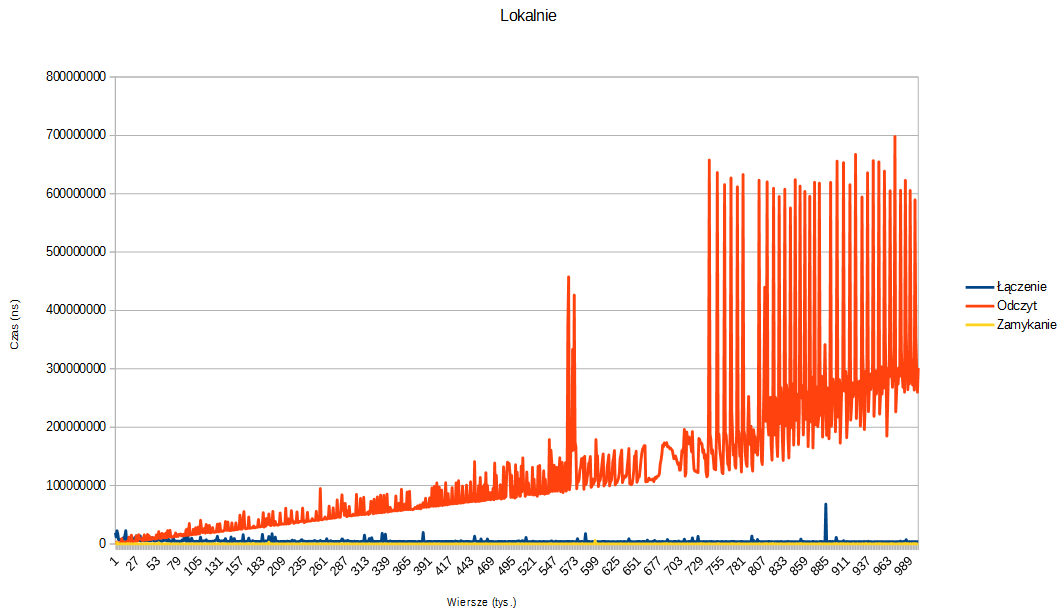
\includegraphics[width=\textwidth]{local1.png}
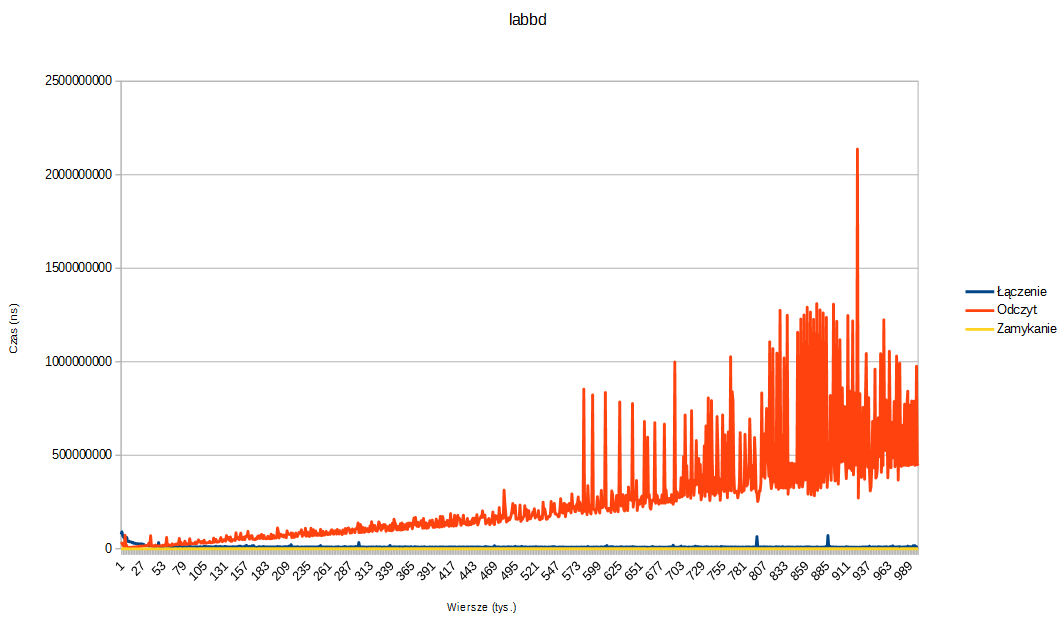
\includegraphics[width=\textwidth]{lab1.png}

Jak widać, czas łączenia jest znikomy w porównaniu do pobierania danych i niewiele z wykresu wynika. Zobaczmy teraz dokładniejsze wykresy:

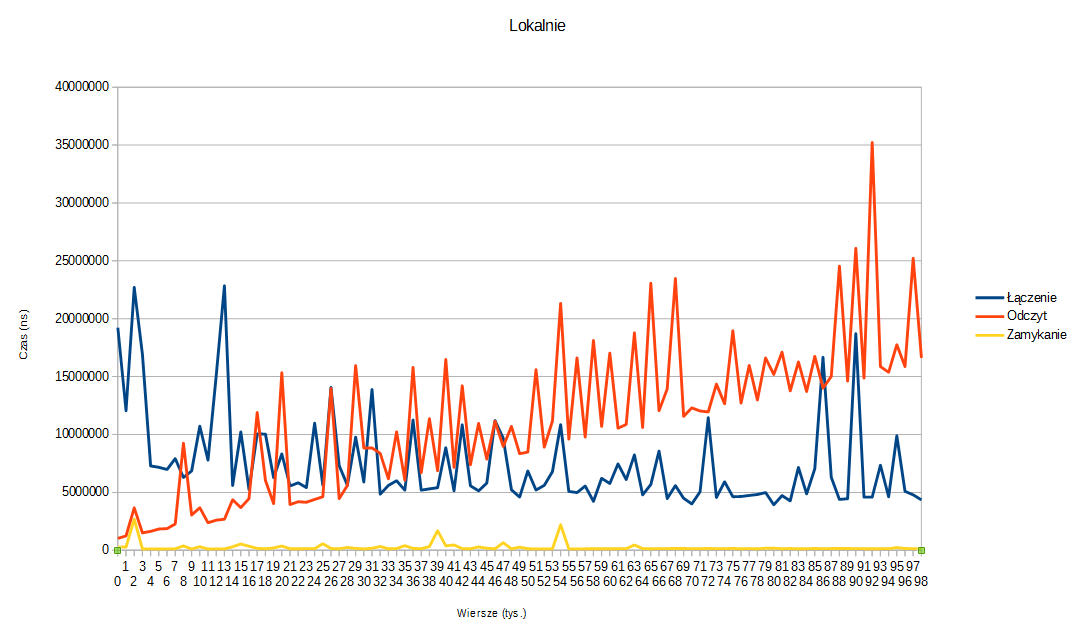
\includegraphics[width=\textwidth]{local2.png}
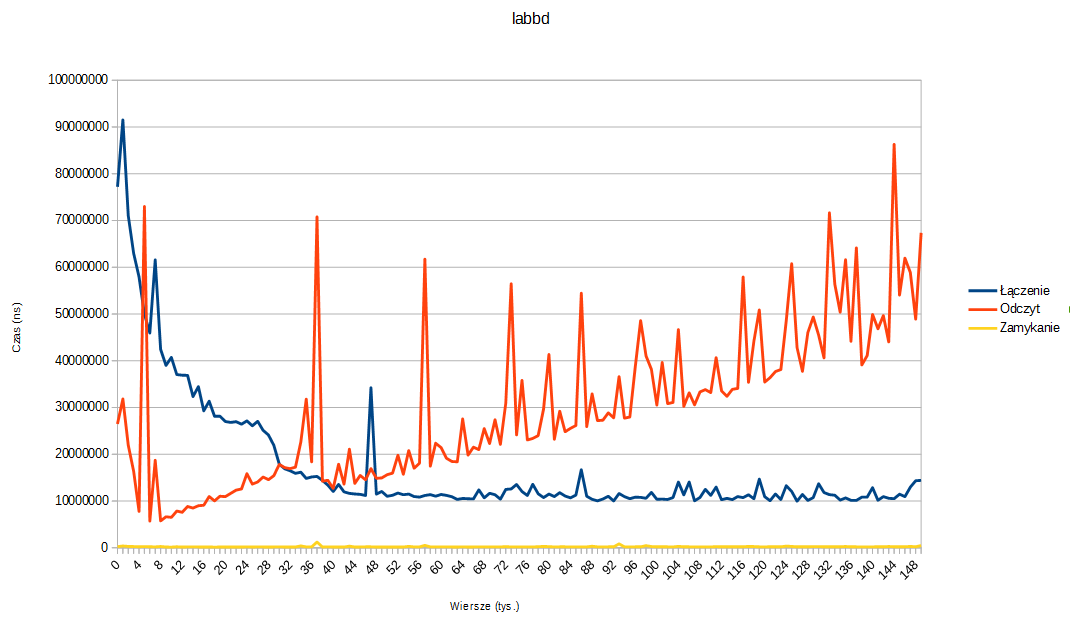
\includegraphics[width=\textwidth]{lab2.png}

Wykresy są dość nieregularne, zdarzają się bardzo duże odchylenia od typowego czasu odczytu. Na komputerze lokalnym wynoszą one zazwyczaj dwukrotność oczekiwanego czasu, na komputerze zdalnym też, ale tutaj maksimum wynosi czterokrotność. Oczekiwany czas odczytu miliona wierszy wynosi ok. 0,3 s na komputerze lokalnym i 0,6 s na labbd.

Ciekawsze są wyniki z mniejszego przedziału. W przypadku łączenia z zdalnym hostem użyłem dłuższej serii by uwypuklić ciekawą zależność. Czas pierwszego łączenia zajmuje aż 90 ms by spaść do 10 ms po wykonaniu 50-ciu iteracji testu. Wygląda to tak, jakby baza danych musiała się ,,rozgrzać". Być może ma to jakiś związek z dynamicznie regulowaną ilością procesów wykonujących zapytania, socketów, wątków albo jakimś cache. Czas łączenia z lokalnym hostem zajmuje jakieś 5 do 10 ms. 

Odpowiadając na pytanie postawione we wstępie do rozdziału, wystarczy pobrać 50 wierszy z tabeli (właściwie to liczb typu integer) by czas łączenia z bazą danych przestał dominować. W ramach ciekawostki zmierzyłem też czas zamykania połączenia. Wygląda na to, że nie są stosowane tutaj żadne wyrafinowane protokoły.

\end{document}

